\documentclass[a4paper, 10pt]{ctexbook} %中文支持
\usepackage{float}              %防止浮动元素浮动
\usepackage{rotating}           %旋转图片用的
\usepackage{hyperref}
\usepackage{amsfonts}           %对某一些字体之支持
\usepackage[]{amsmath}          %数学公式
\usepackage{amsthm}             %定义, 定理, 证明, 例子这些环境的支持
%使用方法:
%\newtheorem{environment name}{caption}
%比如 \newtheorem{example}{这是例子}
%效果 \begin{example} xxx \end{example} -> 这是例子 1 xxx
%proof就不需要了
\usepackage{graphicx}           %用来插入图片
\usepackage[left=1.25in,right=1.25in,top=1in,bottom=1in]{geometry}   %用来排版的
\usepackage[]{color}            %用来给部分文本上色的
\usepackage{algorithm}          %用来写伪代码的
\usepackage{algorithmic}        %同上
\usepackage{minted}
\usepackage{amssymb}            %用来加入一些数学符号, 比如说 $\varnothing$
\usepackage{fontspec}           %不知道用来干嘛的
\setmonofont{Ubuntu Mono}       %?
\usemintedstyle{custommanni}    %设置minted插入代码的风格

\newtheorem{theorem}{定理}
\newtheorem{example}{Example}
\newtheorem{definition}{定义}
\newtheorem{lemma}{引理}
\newtheorem{proposition}{命题}
\begin{document}
\tableofcontents
\chapter{深度优先搜索和广度优先搜索}
我们以前接触过这两位, 是在学习树的时候.

与其说是两种策略, 不如说是使用了两种数据结构. 
深度优先是栈, 而广度优先是队列.

\section{BFS}
下面给出BFS的框架:

\begin{minted}[mathescape, 
                linenos, 
                numbersep=5pt,
                gobble=2,
                frame=lines,
                framesep=2mm]{c++}
    // 构造由根组成的队列 Q
    if Q 中的第一个元素 x 是目标节点
        stop
    else 
        从 Q 中删除 x, 将 x 的所有子节点放进 Q 中.
    if Q == NULL 
        return failed;
    else goto 2
\end{minted}
虽然使用了 \verb|goto| 但也算是简洁了, 其实用 \verb|while| 也很简洁. 
我们说这里的关键就是队列, 其特点就是先进先出. 
对于节点 $x$ , 我们将其子节点放入队列, 这些子节点都搞定之后才会继续搞其他的子节点.

\section{DFS}
区别在于使用了栈.
\begin{minted}[mathescape, 
                linenos, 
                numbersep=5pt,
                gobble=2,
                frame=lines,
                framesep=2mm]{c++}
    // 构造由根组成的栈 S
    if S 中的第一个元素 x 是目标节点
        stop
    else 
        Pop (S) ; 
        Push (s); // 将 S 的子节点压进栈.
    if S == NULL 
        return failed;
    else goto 2
\end{minted}
\chapter{搜索的优化}
\section{爬山法}
基本思想: 
在DFS的过程中, 使用贪心法确定搜索的方向. 爬山策略使用 ``启发式测度'' \footnote{什么几把名字} 来排序节点优先程度. 

这里笔者拒绝使用 ``启发式测度'', 这个听起来很几把无语的词语. 因为这个和测度毫无关系.

我们通过 $f$ 来测量某一个节点, 我们说, 越接近某一值 $a$ 则该节点距离正确答案就越近, 可以按照这一标准来排序节点. 

将当前节点 $x$ 的子节点压进栈的时候, 按照上面给出的排列顺序压进栈. 

于是乎, 我们的算法思路就是这样:
\begin{minted}[mathescape, 
                linenos, 
                numbersep=5pt,
                gobble=2,
                frame=lines,
                framesep=2mm]{c++}
    // 构造由根组成的栈 S
    if S 中的第一个元素 x 是目标节点
        stop
    else 
        Pop (S) ; 
        Push (s); // 将 x 的子节点按照给出的排列顺序压入栈.
    if S == NULL 
        return failed;
    else goto 2
\end{minted}

我们能够明显地看出, 这个搜索策略并不一定是最优的解, 因为这只是一个贪心选择, 我们的问题不一定满足贪心选择性. 

接下来我们要修改的话, 就是考虑到全局的节点.
\section{Best-First 搜索}

类似的, 我们有给出一个函数 $f$ 来考察节点的优先程度.

基本思想: 
\begin{itemize}
    \item 结合深度优先和广度优先的优点
    \item 根据函数 $f$ 在目前产生的所有节点中选择具有最优的节点进行扩展 \footnote{扩展又是什么意思? 我不是说故意挑刺, 但是你不能总是突然冒出一个自己编篡的词语, 然后又不解释是什么意思}
    \item 选择了全局最优解, 而爬山只是局部最优.
\end{itemize}
\begin{minted}[mathescape, 
                linenos, 
                numbersep=5pt,
                gobble=2,
                frame=lines,
                framesep=2mm]{c++}
    依照 f 的值为比较的key, 构造出一个堆, 先是构造只有起点 r 的堆
    if H 的根 x 是目标节点 then stop;
    delete_max(H);  将 x 的子节点插入heap;
    if H == NULL then failed;
    else goto 2
\end{minted}
\section{分支界限}
TODO
基本思想: 
\begin{itemize}
    \item 上述方法很难用于求解优化问题 \footnote{为什么}
    \item 分支界限策略可以有效地求解组合优化问题. 
    \item 发现优化解的一个界限, 缩小解空间, 提高求解的效率 \footnote{你在说什么}
\end{itemize}

我们这里的例子是这样的
\begin{figure}[H]
    \centering
    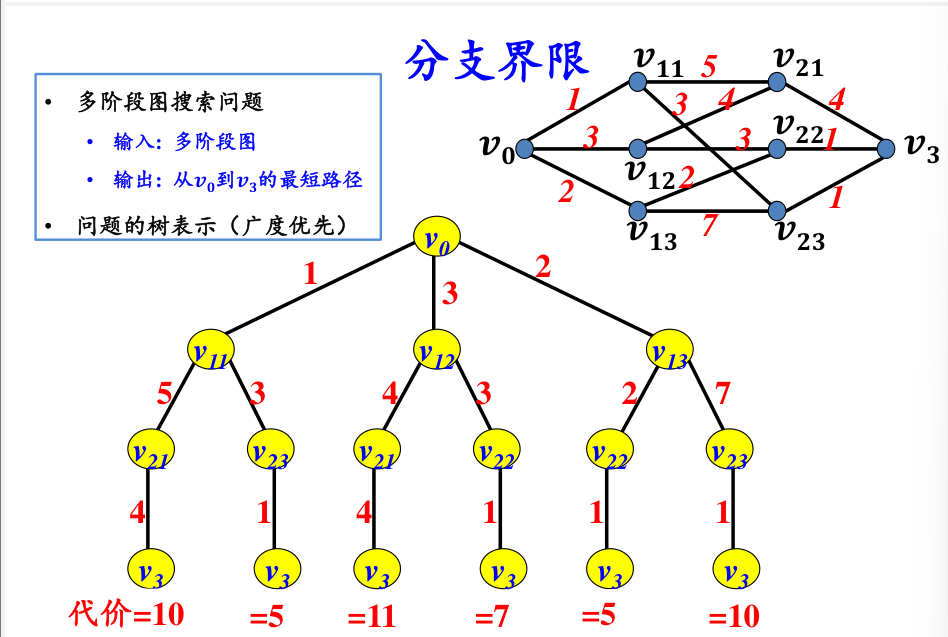
\includegraphics[scale=0.5]{ss1.png}
    \caption{例子}
\end{figure}
\begin{itemize}
    \item[1] 使用爬山策略, 找出一个路径(选择权重最小的边), 1 3 1 这条路
    \item[2] 根据这个解, 进行剪枝. 已知这个路径的长度是 5 , 我们将上一层节点中大于 5 的节点剪去. 这就是缩小了解的范围.  
\end{itemize}

我的评价: 这讲的什么几把, 指ppt 

剪完了然后呢? 难道是根据best-first再搜索一边吗? 
搞不懂捏. 
\chapter{剪枝方法与人员安排问题}
\section{问题定义}

$\mathbf{input}:$ P for person, $P = \left\{P_1 , \cdots  , P_n\right\}$ 是 $n$ 个人的集合. 

人员安排的问题之定义实际上是这样, 我们有一个工作的集合, 他是一个偏序集, 我们将其进行一个拓扑排序, 
比如说 $\left\{J_{i_{k}}\right\}$ 这是排序中的第 $k$ 个工作, 意思就是这个工作由第 $k$ 个人来担任. 

同时给出了一个矩阵 $\left(X_{ij}\right)$ , $X_{ij}$ 的意思是, 第 $i$ 个人分配了第 $j$ 个工作所需要的时间. 

\begin{figure}[H]
    \centering
    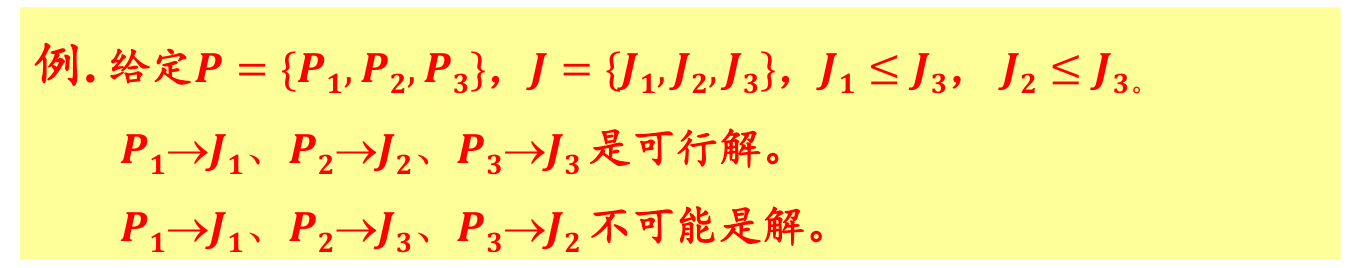
\includegraphics[scale = 0.5]{ss2.png}
    \caption{一个例子}
\end{figure}

于是说, 我们的目的就是要遍历所有的拓扑排序, 从中找到一个最优解, 总体来说这是一个遍历的过程. 我们可以回想以前是怎么找拓扑排序的: 每次选择一个 ``没有前序元素的'' 的元素, 作为当前根节点的子节点. 
对于这些获得的子节点也是使用这样方法, 也就是递归地处理子节点. 

1.  生成空树根 

2. 选择偏序集中没有前序元素的元素, 作为当前根节点的子节点

3. For root 的每一个子节点, do 

4. S =     S - {v}

5.  将 $v$ 作为根, 递归地处理 $S$

我们这就生成了一个拓扑排序对应的树, 这个树上, 从根节点到叶子的一条路就是一个拓扑排序. 我们当然可以对这棵树上的搜索进行优化. 
\section{算法的优化: 针对代价矩阵做出的优化}
\begin{proposition}
    将代价矩阵的一行或者一列, 减去同一个数字, 不影响优化解的求解.
\end{proposition}
\begin{itemize}
    \item 代价矩阵的每行减去同一个数, 使得每一行以及每一列是找有一个零, 其余元素非负. 
    \item 减数的和是解的一个下界. 
\end{itemize}    

\begin{figure}
    \centering
    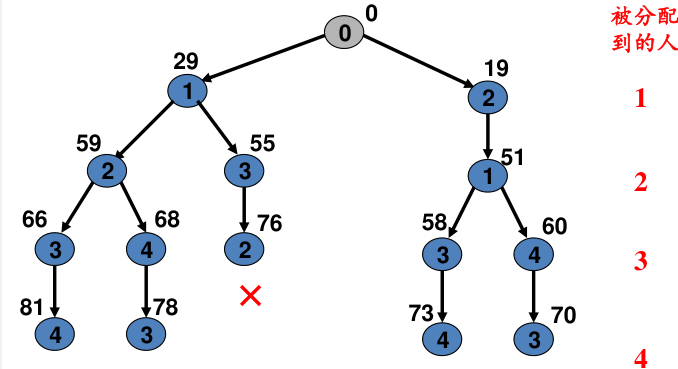
\includegraphics[scale = 0.5]{ss3.png}
    \caption{优化前的树}
\end{figure}

\begin{figure}
    \centering
    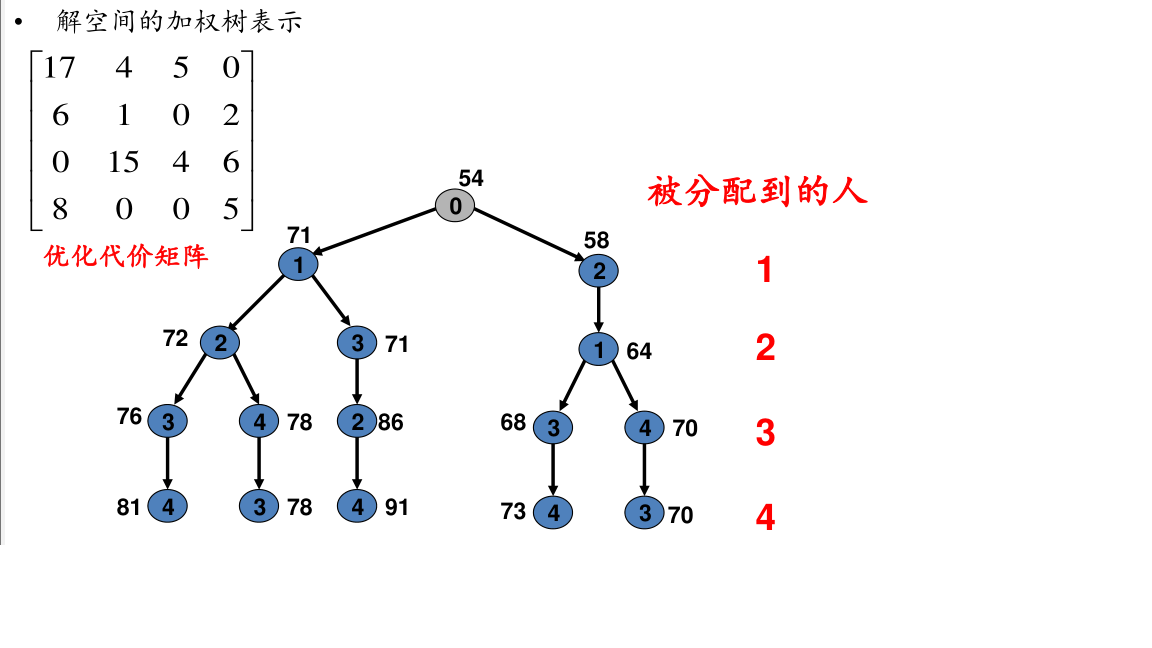
\includegraphics[scale =0.5]{ss4.png}
    \caption{优化后的树}
\end{figure}

优化之后, 根节点的值为前面计算的下界. 

总之, 通过分支界限法, 来剪枝, 优化之后的树能够有效的进行剪枝
\begin{figure}
    \centering
    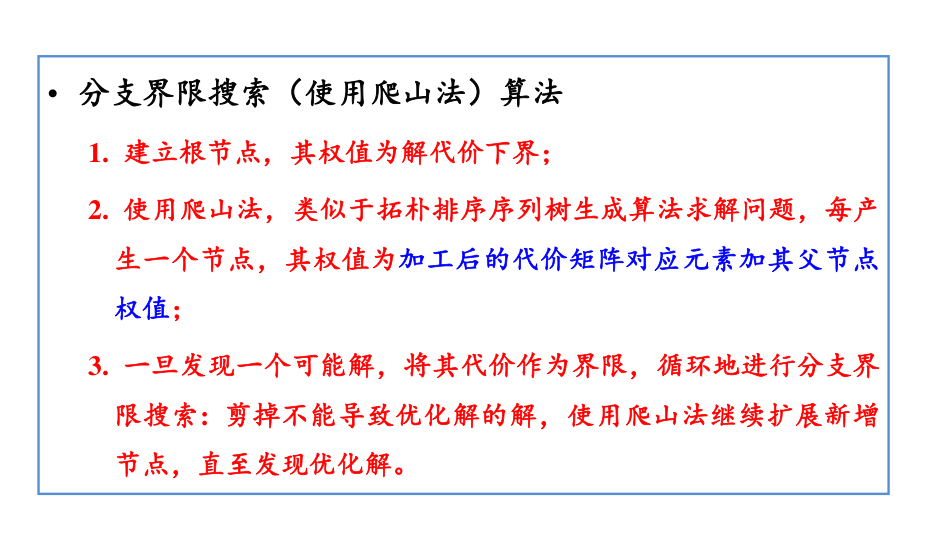
\includegraphics[scale = 0.5]{ss5.png}
\end{figure}
\chapter{旅行商问题}
todo

我是想问, 你能不能去吃粪?
\chapter{A*算法}
todo
\end{document} 